\documentclass{article}
\usepackage{graphicx} % Required for inserting images
\usepackage[utf8]{inputenc}
\usepackage[portuguese]{babel}
\usepackage{graphicx}
\usepackage{listings}
\usepackage{hyperref}

\title{\textbf{Relatório LI}}
\author{a22999 - Joana Pimenta
   \and a23000 - Diogo Marques
   \and a23135 - Miguel Simões}

\date{December 2023}

\begin{document}

\maketitle

\newpage

\section*{Índice de Conteúdos}
\subsection*{\tableofcontents}


\newpage

\section*{Índice de Figuras}

\subsection*{\listoffigures}
\subsection*{\listoftables}

\newpage

\section{Introdução}
 O presente relatório aborda de forma detalhada o desenvolvimento de uma aplicação de gabinete de nutrição com o objetivo de gerenciar de forma eficiente e organizada os dados dos pacientes, os planos nutricionais e o consumo de alimentos. A aplicação será implementada em linguagem \emph{C}, seguindo o paradigma de programação imperativa. \\ \\ Além de apresentar as funcionalidades básicas da aplicação, o relatório também oferecerá uma visão sobre o desenvolvimento do sistema, destacando as etapas do processo e as decisões tomadas durante a implementação. Adicionalmente, serão demonstrados casos aplicados para testar e validar a aplicação, garantindo sua funcionalidade e confiabilidade em diferentes cenários. 
\\ \\Para a gestão do projeto, será utilizado um repositório do \emph{Github} para o controle de versionamento e colaboração entre os membros da equipe. Além disso, para garantir uma documentação completa e detalhada da aplicação, optamos por utilizar a ferramenta \emph{Doxygen}, para nos permitir gerar automaticamente documentação a partir do código-fonte.

\newpage



\newpage
\section{Funcionalidades Implementadas}

\subsection{Menu Principal}
De forma a facilmente aceder todas as funcionalidades do sistema foi feito um Menu Principal que serve como \emph{hub} da aplicação. O mesmo tem 8 opções, contando com a de saída que para o programa. \\O Menu Principal é uma parte fundamental da aplicação, pois permite que o utilizador navegue de forma intuitiva e eficiente pelas diferentes funcionalidades disponíveis. \\Além disso, o Menu Principal foi projetado de maneira clara e autoexplicativa, garantindo que todas as opções sejam facilmente identificáveis. Com isso, o utilizador pode explorar todas as opções e recursos do sistema de forma simples.\\

\begin{figure}[h]
    \centering
    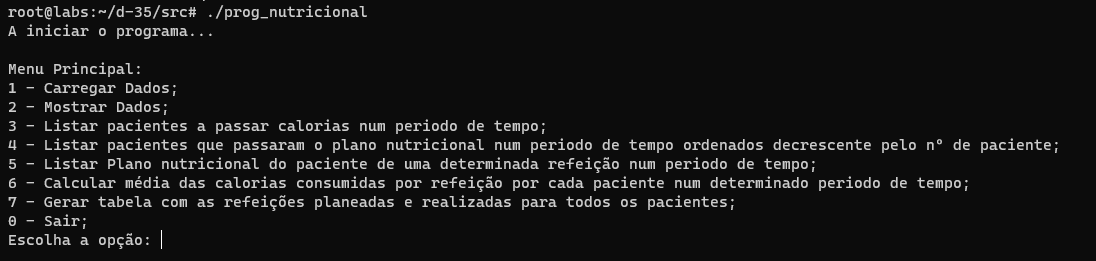
\includegraphics[width=0.9\linewidth]{MenuPrincipal.png}
    \caption{Consola do Menu Principal}
    \label{fig+:enter-label}
\end{figure}

\subsection{Carregamento de Dados dos Pacientes}
Para funcionamento da aplicação a mesma precisa de ser carregada com dados que serão trabalhados em para todas as funcionalidades. Além disso, é importante ressaltar que esses dados devem ser processados de forma adequada para garantir o pleno desempenho das funcionalidades.

\begin{figure}[h]
    \centering
    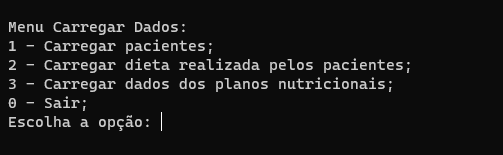
\includegraphics[width=0.6\linewidth]{menuCarregarDados.png}
    \caption{Consola do Menu Carregar Dados}
    \label{fig:enter-label}
\end{figure}

\newpage

\subsubsection{Ficheiro de Dados dos Pacientes}
O primeiro passo envolve o carregamento de dados dos pacientes a partir de um ficheiro de texto. Cada linha do ficheiro contém informações como \textit{id} do paciente, nome e telefone. \\O mesmo foi feito através da função \textbf{“carregarClientes”}, que verifica se já existe uma lista com dados de clientes. \\Caso se verifique oferece ao utilizador a opção de sobrescrever a lista já existente ou simplesmente carregar novos dados. Após isso pede o \emph{path} do ficheiro a carregar e caso o mesmo seja válido percorre-o adicionando os dados à lista. \\Caso não exista realiza apenas a segunda parte.\\

\begin{figure}[h]
    \centering
    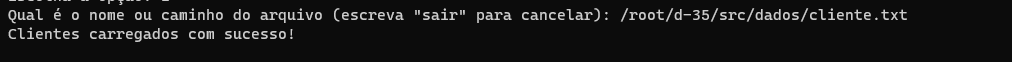
\includegraphics[width=0.8\linewidth]{CarregarCliente.png}
    \caption{Consola Carregamento de Dados dos Pacientes}
    \label{fig:enter-label}
\end{figure}

\subsubsection{Ficheiro de Dieta dos Pacientes}
Além disso, o conteúdo de um segundo ficheiro de texto é carregado, contendo informações sobre a dieta realizada por cada paciente, incluindo \textit{id} do paciente, data, refeição, alimento e calorias. \\Este carregamento foi feito através da função \textbf{“carregarDietasRealizadas”}. \\ Se existir oferece ao utilizador a opção de sobrescrever a lista já existente ou simplesmente carregar novos dados. Pede então o caminho do ficheiro e se o mesmo é válido percorre o ficheiro e adiciona os dados à lista. \\Caso não exista realiza apenas a segunda parte.\\

\begin{figure}[h]
    \centering
    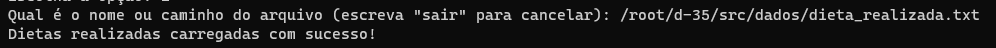
\includegraphics[width=0.8\linewidth]{CarregarDieta.png}
    \caption{Consola Carregamento de Dieta dos Pacientes}
    \label{fig:enter-label}
\end{figure}

\subsubsection{Ficheiro de Planos Nutricionais}
O conteúdo de um terceiro ficheiro de texto é também carregado, contendo dados dos planos nutricionais ajustados ao perfil de cada paciente. Cada linha identifica o paciente, a data de Inicio, data de Fim, o tipo de refeição e as calorias mínimas e máximas permitidas. Foi adicionada a coluna de data de Fim pois no ponto 6 do enunciado o mesmo foi referido e chegou-se ao consenso que faria sentido ela entrar aqui. \\Para carregar estes dados passa pela função \textbf{“carregarPlanosNutricionais”}. \\ Caso o mesmo exista apresenta ao utilizador a opção de sobrescrever a lista já existente ou simplesmente carregar novos dados. Requer o \emph{path} do ficheiro e caso o mesmo seja válido percorre o ficheiro e adiciona os dados à lista. \\Caso não exista realiza apenas a segunda parte.\\

\begin{figure}[h]
    \centering
    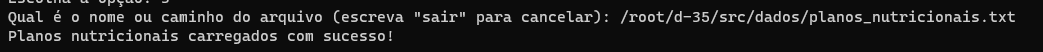
\includegraphics[width=0.8\linewidth]{CarregarPlanos.png}
    \caption{Consola Carregamento de Planos Nutricionais}
    \label{fig:enter-label}
\end{figure}

\subsubsection{Apresentação dos Dados Carregados no Sistema}
Para o utilizador poder visualizar dentro do programa os dados previamente inseridos, foi criado um menu para aceder os mesmos.

\begin{figure}[h]
    \centering
    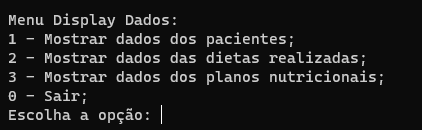
\includegraphics[width=0.6\linewidth]{MenuMostrarDados.png}
    \caption{Consola do Menu de \emph{Display} dos Dados Carregados}
    \label{fig:enter-label}
\end{figure}

Tem então a opção de \emph{Display} dos 3 tipos de carregamentos executáveis.

\begin{figure}[hbt!]
    \centering
    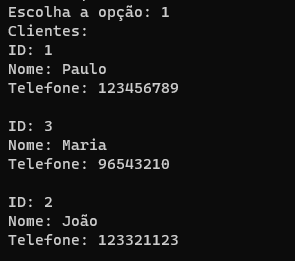
\includegraphics[width=0.4\linewidth]{DisplayClientes.png}
    \caption{Consola de \emph{Display} de Pacientes}
    \label{fig:enter-label}
\end{figure}

\begin{figure}[hbt!]
    \centering
    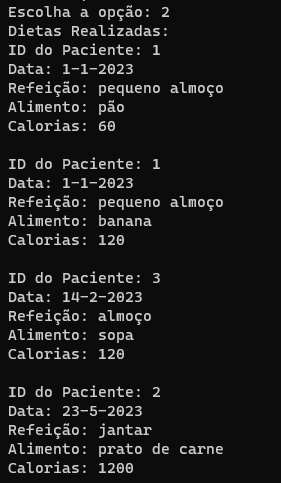
\includegraphics[width=0.3\linewidth]{DispalyDietas.png}
    \caption{Consola de \emph{Display} de Dietas Realizadas}
    \label{fig:enter-label}
\end{figure}

\begin{figure}[hbt!]
    \centering
    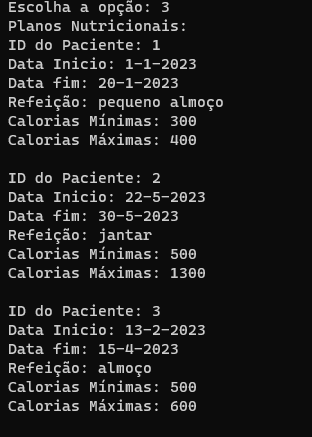
\includegraphics[width=0.4\linewidth]{DisplayPlanos.png}
    \caption{Consola de \emph{Display} de Planos Nutricionais}
    \label{fig:enter-label}
\end{figure}

\newpage

\subsection{Número de Pacientes com Excesso de Calorias}
Implementou-se a funcionalidade de apresentar o número de pacientes que ultrapassaram uma determinada quantidade de calorias em um período específico. Atingiu-se isso através da função \textbf{"clientesPassaramCaloriasPeriodoTempo"}. Decompondo esta função deparámo-nos inicialmente, com uma solicitação ao utilizador para inserir as datas de início e fim do período desejado, bem como o valor mínimo de calorias a ser considerado. A função realiza verificações para garantir que as listas de clientes e dietas estejam carregadas antes de prosseguir.\\

Durante a execução, a função itera sobre a lista de clientes, acompanhando o total de calorias consumidas por cada um no período especificado. Simultaneamente, um \emph{loop} interno percorre as dietas realizadas, acumulando as calorias correspondentes àquele cliente e período. Se o total de calorias consumidas por um cliente atingir ou ultrapassar o valor mínimo especificado, o contador total é incrementado.\\

Ao final da execução, a função exibe o número total de clientes que ultrapassaram o limite de calorias durante o intervalo de tempo determinado. Esse resultado proporciona uma visão prática e quantificada do comportamento alimentar dos clientes, sendo útil para avaliação e intervenção nutricional.\\

\begin{figure}[h]
    \centering
    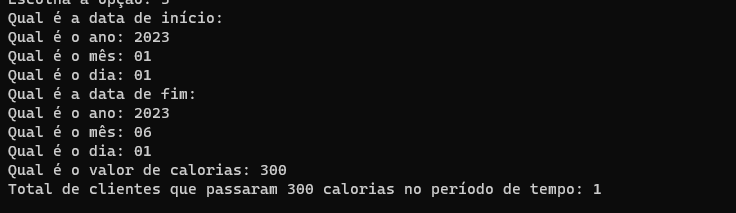
\includegraphics[width=0.8\linewidth]{Ponto2.png}
    \caption{Consola de execução de Número de Pacientes com Excesso de Calorias}
    \label{fig:enter-label}
\end{figure}

\subsection{Listagem de Pacientes com Calorias Fora do Intervalo}
Foi implementada a listagem dos pacientes, ordenada por ordem decrescente do número do paciente, que realizaram alguma refeição com quantidade de calorias fora do intervalo permitido pelo plano nutricional através da função \textbf{"clientesPassaramPlanoNutricionalPeriodoTempoDecrescente"}.\\ A função inicia criando uma nova lista de clientes, \textbf{"listaClienteDecrescente"}, que será utilizada para armazenar os clientes que não cumpriram o plano nutricional durante o período estipulado.

Em seguida, são realizadas verificações iniciais para garantir que as listas de clientes, planos nutricionais e dietas realizadas estejam carregadas. Caso contrário, a função imprime mensagens correspondentes e encerra sua execução.\\

O utilizador é então solicitado a inserir as datas de início e fim do período desejado, seguido pela validação do intervalo de datas. Caso o intervalo seja inválido, é pedido ao utilizador para inserir novamente até o intervalo ser válido.

A função entra em um \emph{loop} que itera sobre cada cliente na lista de clientes. Para cada cliente, outro \emph{loop} é iniciado para percorrer a lista de planos nutricionais. Dentro verifica-se se o plano nutricional pertence ao cliente atual e está dentro do intervalo de datas especificado. Se essas condições forem atendidas, um terceiro \emph{loop} é iniciado para percorrer as dietas realizadas relacionadas a esse plano nutricional.\\ 

O total de calorias consumidas por refeição é calculado e comparado aos limites do plano nutricional. Se o total de calorias estiver fora dos limites, o cliente é inserido na lista \textbf{"listaClienteDecrescente"}.

Ao final do processo de iteração, a lista \textbf{"listaClienteDecrescente"} é ordenada em ordem decrescente com base no número de paciente. A função então exibe as informações dos clientes que não cumpriram o plano nutricional durante o período estipulado, incluindo o \textit{ID}, nome e telefone.\\

Se nenhum cliente atender aos critérios, uma mensagem indicando que nenhum cliente ultrapassou o plano nutricional no período de tempo é impressa. Por fim, a lista temporária é liberada da memória.

\begin{figure}[hbt!]
    \centering
    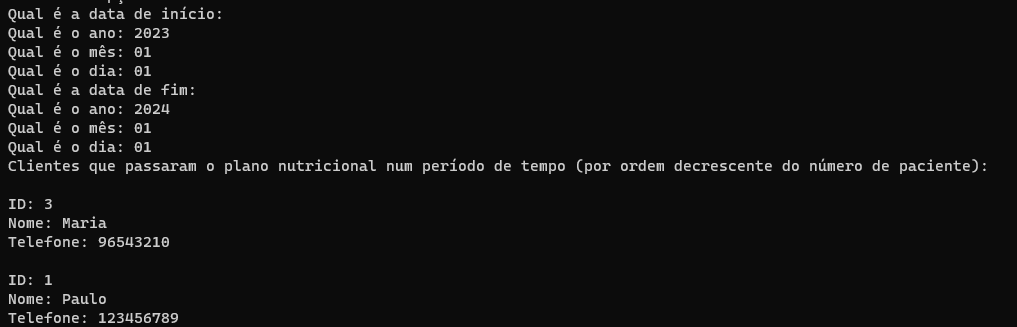
\includegraphics[width=0.9\linewidth]{Ponto3.png}
    \caption{Consola de execução da Listagem de Pacientes com Calorias Fora do Intervalo}
    \label{fig:enter-label}
\end{figure}

\subsection{Listar Plano Nutricional de um Paciente}
É possível listar o plano nutricional de um paciente para determinada refeição ao longo de um período específico.

A função \textbf{"listarPlanoNutricionalPacienteRefeicaoPeriodoTempo"} inicia fazendo verificações para garantir que as listas de clientes e planos nutricionais estejam carregadas. Se alguma delas estiver vazia, a função imprime mensagens correspondentes e encerra sua execução.\\

É pedido ao utilizador que insera as datas de início e fim do período desejado, e a validação do intervalo de datas é realizada. Caso o intervalo seja inválido, o utilizador é requisitado novamente até inserir um intervalo válido.

O utilizador também é solicitado a escolher o tipo de refeição desejado (pequeno almoço, almoço ou jantar) e inserir o \textit{ID} do paciente. A função realiza verificações adicionais para garantir que o tipo de refeição e o \textit{ID} do paciente estejam dentro dos limites válidos.\\

Em seguida, a função entra em um \emph{loop} que itera sobre cada plano nutricional na lista. Para cada plano nutricional, verifica-se se ele pertence ao paciente e está dentro do intervalo de datas e refere-se ao tipo de refeição especificado. Se essas condições forem atendidas, as informações detalhadas do plano nutricional são exibidas, incluindo a data de início, a data de fim, as calorias mínimas e máximas.
Ao final do processo de iteração, a função imprime uma mensagem indicando que nenhuma refeição foi encontrada se nenhum plano nutricional atender aos critérios especificados.
\\ 

\begin{figure}[hbt!]
    \centering
    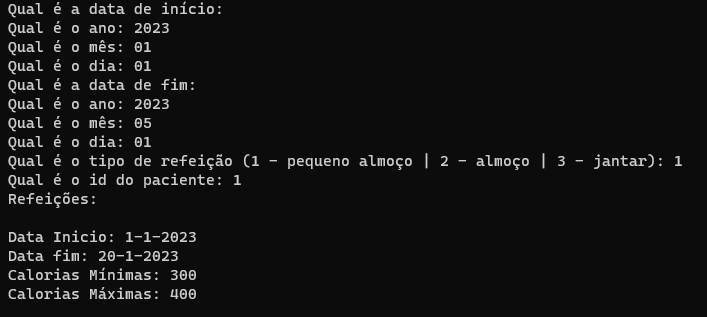
\includegraphics[width=0.9\linewidth]{Ponto4.png}
    \caption{Consola de execução da Listagem do Plano Nutricional de um Paciente}
    \label{fig:enter-label}
\end{figure}

\subsection{Cálculo das Médias de Calorias Consumidas}
A aplicação realiza o cálculo das médias das calorias consumidas por refeição por cada paciente ao longo de um determinado período.
A função \textbf{"calcularMediaCalRefeicaoPassadoPeriodoTempo"} começa por efetuar verificações para garantir que as listas de clientes e dietas realizadas estejam carregadas. Caso alguma delas esteja vazia, a função imprime mensagens correspondentes e encerra sua execução.\\

O utilizador é então solicitado a inserir as datas de início e fim do período desejado, com validação do intervalo de datas. Se o intervalo for inválido, o utilizador é solicitado novamente até inserir um intervalo válido.

A função entra em um \emph{loop} que itera sobre cada cliente na lista. Para cada cliente, outro \emph{loop} é iniciado para percorrer as três refeições possíveis (pequeno almoço, almoço e jantar). Dentro desse ciclo, itera-se sobre a lista de dietas realizadas para verificar se há alguma entrada correspondente à refeição, ao cliente e ao intervalo de datas especificados.\\

Se uma entrada é encontrada, a função calcula a média de calorias consumidas para aquela refeição e imprime as informações do cliente, incluindo o \textit{ID}, nome, tipo de refeição e a média de calorias. Repete-se para todas as refeições em que o cliente teve dietas realizadas durante o período especificado.
Ao final do processo de iteração, a função imprime uma mensagem indicando que não há dados disponíveis se nenhum cliente atender aos critérios especificados.

\begin{figure}[hbt!]
    \centering
    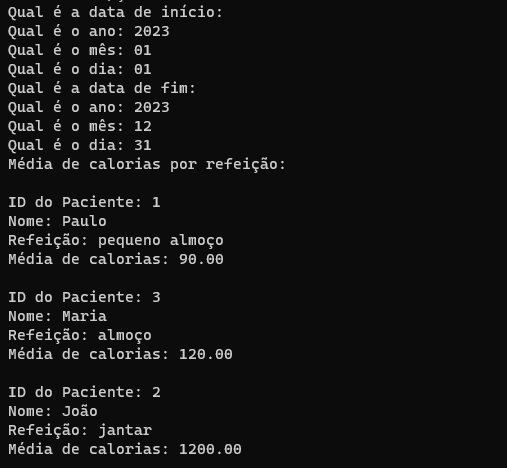
\includegraphics[width=0.8\linewidth]{Ponto5.png}
    \caption{Consola de execução do Cálculo das Médias de Calorias Consumidas}
    \label{fig:enter-label}
\end{figure}


\subsection{Geração da Tabela de Refeições Planeadas e Realizadas}
A tabela apresenta as refeições planeadas e realizadas para todos os pacientes, incluindo informações como número do paciente, nome, tipo de refeição, data de início, data de fim, calorias mínimo, calorias máximo e consumo realizado. A função \textbf{"gerarTabelaRefeicoesPlaneadas"} começa por realizar verificações para garantir que as listas de clientes, planos nutricionais e dietas realizadas estejam carregadas. Se alguma delas estiver vazia, a função imprime mensagens correspondentes e encerra sua execução.\\

Em seguida, a função inicia dois \emph{loops} encadeados: o primeiro itera sobre cada cliente na lista de clientes, e o segundo itera sobre cada plano nutricional na lista de planos nutricionais.

Dentro desses \emph{loops}, a função verifica se há dietas realizadas correspondentes ao paciente e ao plano nutricional. Se sim, ela calcula o total de calorias consumidas e cria uma estrutura \textbf{RefeicoesPlaneadas} para armazenar as informações relevantes. Essa estrutura é então inserida em uma lista \textbf{listaRefeicoesPlaneadas}.\\

A função lida com situações de erro, como falha na inserção de dados na lista ou erros durante a iteração nas listas.
Após a conclusão dos \emph{loops}, a função imprime uma tabela formatada contendo os detalhes das refeições planeadas, incluindo um cabeçalho com as informações relevantes.
Ao final, a função libera a memória alocada para a lista de refeições planeadas e reinicializa essa lista para uso futuro. \\

\begin{figure}[hbt!]
    \centering
    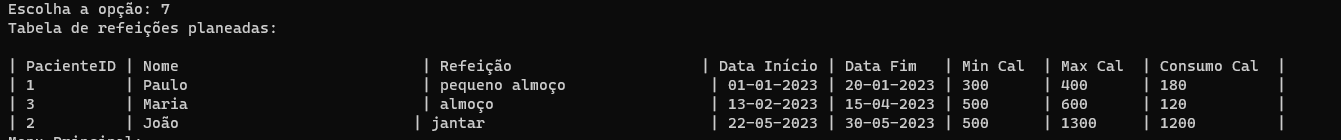
\includegraphics[width=1.1\linewidth]{Ponto6.png}
    \caption{Consola de execução da Tabela de Refeições Planeadas e Realizadas}
    \label{fig:enter-label}
\end{figure}

\newpage
\section{Conclusão}
Conclui-se que foi feita uma boa abordagem ao projeto consoante o enunciado sugerido e que pusemos em pratica as competências adquiridas nas UCs de Programação Imperativa e Laboratórios de Informática. \\

É importante ressaltar que o trabalho em equipe desempenhou um papel fundamental nesse processo, permitindo a troca de ideias, a colaboração mútua e o alcance dos resultados. Nunca tinhamos trabalhado com esta forma de ler arquivos, separados por ";" e tabuladores, o que se apresentou inicialmente como um desafio mas sem muitos contratempos fomos capazes dominar este metódo. O maios desafio, em que tivemos mais dificuldade, foi a parte de manipulação de datas e verificar se o intervalo estava dentro do outro, que também nunca tínhamos trabalhado com, mas ultrapassamos essas complicações e tudo funciona comforme o esperado.\\

O desenvolvimento desta aplicação em linguagem C \cite{Online} proporcionou-nos novos conhecimentos e também novas ferramentas de trabalho, como o \emph{Doxygen}\cite{Doxygen} e a Linguagem \LaTeX \cite{Documentação}, que certamente voltaremos a usar. As funcionalidades implementadas atendem totalmente às necessidades e requisitos descritos no enunciado do projeto portanto crêmos que possa ser considerado um sucesso.

\section{Bibliografia}

\bibliographystyle{plain}
\bibliography{bibliogarfia.bib}

\end{document}


